\documentclass[1p]{elsarticle_modified}
%\bibliographystyle{elsarticle-num}

%\usepackage[colorlinks]{hyperref}
%\usepackage{abbrmath_seonhwa} %\Abb, \Ascr, \Acal ,\Abf, \Afrak
\usepackage{amsfonts}
\usepackage{amssymb}
\usepackage{amsmath}
\usepackage{amsthm}
\usepackage{scalefnt}
\usepackage{amsbsy}
\usepackage{kotex}
\usepackage{caption}
\usepackage{subfig}
\usepackage{color}
\usepackage{graphicx}
\usepackage{xcolor} %% white, black, red, green, blue, cyan, magenta, yellow
\usepackage{float}
\usepackage{setspace}
\usepackage{hyperref}

\usepackage{tikz}
\usetikzlibrary{arrows}

\usepackage{multirow}
\usepackage{array} % fixed length table
\usepackage{hhline}

%%%%%%%%%%%%%%%%%%%%%
\makeatletter
\renewcommand*\env@matrix[1][\arraystretch]{%
	\edef\arraystretch{#1}%
	\hskip -\arraycolsep
	\let\@ifnextchar\new@ifnextchar
	\array{*\c@MaxMatrixCols c}}
\makeatother %https://tex.stackexchange.com/questions/14071/how-can-i-increase-the-line-spacing-in-a-matrix
%%%%%%%%%%%%%%%

\usepackage[normalem]{ulem}

\newcommand{\msout}[1]{\ifmmode\text{\sout{\ensuremath{#1}}}\else\sout{#1}\fi}
%SOURCE: \msout is \stkout macro in https://tex.stackexchange.com/questions/20609/strikeout-in-math-mode

\newcommand{\cancel}[1]{
	\ifmmode
	{\color{red}\msout{#1}}
	\else
	{\color{red}\sout{#1}}
	\fi
}

\newcommand{\add}[1]{
	{\color{blue}\uwave{#1}}
}

\newcommand{\replace}[2]{
	\ifmmode
	{\color{red}\msout{#1}}{\color{blue}\uwave{#2}}
	\else
	{\color{red}\sout{#1}}{\color{blue}\uwave{#2}}
	\fi
}

\newcommand{\Sol}{\mathcal{S}} %segment
\newcommand{\D}{D} %diagram
\newcommand{\A}{\mathcal{A}} %arc


%%%%%%%%%%%%%%%%%%%%%%%%%%%%%5 test

\def\sl{\operatorname{\textup{SL}}(2,\Cbb)}
\def\psl{\operatorname{\textup{PSL}}(2,\Cbb)}
\def\quan{\mkern 1mu \triangleright \mkern 1mu}

\theoremstyle{definition}
\newtheorem{thm}{Theorem}[section]
\newtheorem{prop}[thm]{Proposition}
\newtheorem{lem}[thm]{Lemma}
\newtheorem{ques}[thm]{Question}
\newtheorem{cor}[thm]{Corollary}
\newtheorem{defn}[thm]{Definition}
\newtheorem{exam}[thm]{Example}
\newtheorem{rmk}[thm]{Remark}
\newtheorem{alg}[thm]{Algorithm}

\newcommand{\I}{\sqrt{-1}}
\begin{document}

%\begin{frontmatter}
%
%\title{Boundary parabolic representations of knots up to 8 crossings}
%
%%% Group authors per affiliation:
%\author{Yunhi Cho} 
%\address{Department of Mathematics, University of Seoul, Seoul, Korea}
%\ead{yhcho@uos.ac.kr}
%
%
%\author{Seonhwa Kim} %\fnref{s_kim}}
%\address{Center for Geometry and Physics, Institute for Basic Science, Pohang, 37673, Korea}
%\ead{ryeona17@ibs.re.kr}
%
%\author{Hyuk Kim}
%\address{Department of Mathematical Sciences, Seoul National University, Seoul 08826, Korea}
%\ead{hyukkim@snu.ac.kr}
%
%\author{Seokbeom Yoon}
%\address{Department of Mathematical Sciences, Seoul National University, Seoul, 08826,  Korea}
%\ead{sbyoon15@snu.ac.kr}
%
%\begin{abstract}
%We find all boundary parabolic representation of knots up to 8 crossings.
%
%\end{abstract}
%\begin{keyword}
%    \MSC[2010] 57M25 
%\end{keyword}
%
%\end{frontmatter}

%\linenumbers
%\tableofcontents
%
\newcommand\colored[1]{\textcolor{white}{\rule[-0.35ex]{0.8em}{1.4ex}}\kern-0.8em\color{red} #1}%
%\newcommand\colored[1]{\textcolor{white}{ #1}\kern-2.17ex	\textcolor{white}{ #1}\kern-1.81ex	\textcolor{white}{ #1}\kern-2.15ex\color{red}#1	}

{\Large $\underline{12a_{1209}~(K12a_{1209})}$}

\setlength{\tabcolsep}{10pt}
\renewcommand{\arraystretch}{1.6}
\vspace{1cm}\begin{tabular}{m{100pt}>{\centering\arraybackslash}m{274pt}}
\multirow{5}{120pt}{
	\centering
	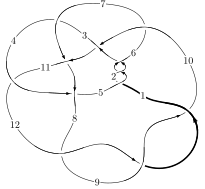
\includegraphics[width=112pt]{../../../GIT/diagram.site/Diagrams/png/2010_12a_1209.png}\\
\ \ \ A knot diagram\footnotemark}&
\allowdisplaybreaks
\textbf{Linearized knot diagam} \\
\cline{2-2}
 &
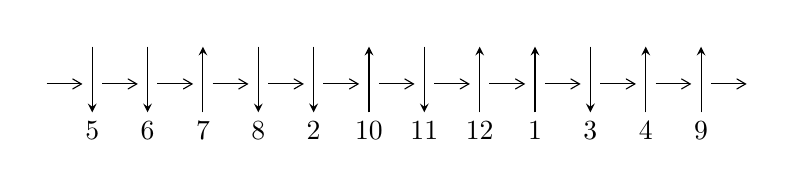
\begin{tikzpicture}[x=20pt, y=17pt]
	% nodes
	\node (C0) at (0, 0) {};
	\node (C1) at (1, 0) {};
	\node (C1U) at (1, +1) {};
	\node (C1D) at (1, -1) {5};

	\node (C2) at (2, 0) {};
	\node (C2U) at (2, +1) {};
	\node (C2D) at (2, -1) {6};

	\node (C3) at (3, 0) {};
	\node (C3U) at (3, +1) {};
	\node (C3D) at (3, -1) {7};

	\node (C4) at (4, 0) {};
	\node (C4U) at (4, +1) {};
	\node (C4D) at (4, -1) {8};

	\node (C5) at (5, 0) {};
	\node (C5U) at (5, +1) {};
	\node (C5D) at (5, -1) {2};

	\node (C6) at (6, 0) {};
	\node (C6U) at (6, +1) {};
	\node (C6D) at (6, -1) {10};

	\node (C7) at (7, 0) {};
	\node (C7U) at (7, +1) {};
	\node (C7D) at (7, -1) {11};

	\node (C8) at (8, 0) {};
	\node (C8U) at (8, +1) {};
	\node (C8D) at (8, -1) {12};

	\node (C9) at (9, 0) {};
	\node (C9U) at (9, +1) {};
	\node (C9D) at (9, -1) {1};

	\node (C10) at (10, 0) {};
	\node (C10U) at (10, +1) {};
	\node (C10D) at (10, -1) {3};

	\node (C11) at (11, 0) {};
	\node (C11U) at (11, +1) {};
	\node (C11D) at (11, -1) {4};

	\node (C12) at (12, 0) {};
	\node (C12U) at (12, +1) {};
	\node (C12D) at (12, -1) {9};
	\node (C13) at (13, 0) {};

	% arrows
	\draw[->,>={angle 60}]
	(C0) edge (C1) (C1) edge (C2) (C2) edge (C3) (C3) edge (C4) (C4) edge (C5) (C5) edge (C6) (C6) edge (C7) (C7) edge (C8) (C8) edge (C9) (C9) edge (C10) (C10) edge (C11) (C11) edge (C12) (C12) edge (C13) ;	\draw[->,>=stealth]
	(C1U) edge (C1D) (C2U) edge (C2D) (C3D) edge (C3U) (C4U) edge (C4D) (C5U) edge (C5D) (C6D) edge (C6U) (C7U) edge (C7D) (C8D) edge (C8U) (C9D) edge (C9U) (C10U) edge (C10D) (C11D) edge (C11U) (C12D) edge (C12U) ;
	\end{tikzpicture} \\
\hhline{~~} \\& 
\textbf{Solving Sequence} \\ \cline{2-2} 
 &
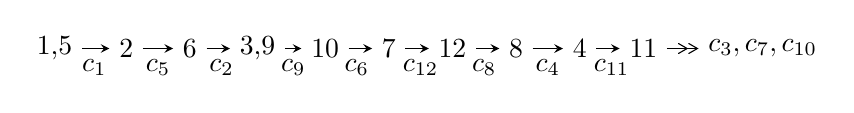
\begin{tikzpicture}[x=23pt, y=7pt]
	% node
	\node (A0) at (-1/8, 0) {1,5};
	\node (A1) at (1, 0) {2};
	\node (A2) at (2, 0) {6};
	\node (A3) at (49/16, 0) {3,9};
	\node (A4) at (33/8, 0) {10};
	\node (A5) at (41/8, 0) {7};
	\node (A6) at (49/8, 0) {12};
	\node (A7) at (57/8, 0) {8};
	\node (A8) at (65/8, 0) {4};
	\node (A9) at (73/8, 0) {11};
	\node (C1) at (1/2, -1) {$c_{1}$};
	\node (C2) at (3/2, -1) {$c_{5}$};
	\node (C3) at (5/2, -1) {$c_{2}$};
	\node (C4) at (29/8, -1) {$c_{9}$};
	\node (C5) at (37/8, -1) {$c_{6}$};
	\node (C6) at (45/8, -1) {$c_{12}$};
	\node (C7) at (53/8, -1) {$c_{8}$};
	\node (C8) at (61/8, -1) {$c_{4}$};
	\node (C9) at (69/8, -1) {$c_{11}$};
	\node (A10) at (11, 0) {$c_{3},c_{7},c_{10}$};

	% edge
	\draw[->,>=stealth]	
	(A0) edge (A1) (A1) edge (A2) (A2) edge (A3) (A3) edge (A4) (A4) edge (A5) (A5) edge (A6) (A6) edge (A7) (A7) edge (A8) (A8) edge (A9) ;
	\draw[->>,>={angle 60}]	
	(A9) edge (A10);
\end{tikzpicture} \\ 

\end{tabular} \\

\footnotetext{
The image of knot diagram is generated by the software ``\textbf{Draw programme}" developed by Andrew Bartholomew(\url{http://www.layer8.co.uk/maths/draw/index.htm\#Running-draw}), where we modified some parts for our purpose(\url{https://github.com/CATsTAILs/LinksPainter}).
}\phantom \\ \newline 
\centering \textbf{Ideals for irreducible components\footnotemark of $X_{\text{par}}$} 
 
\begin{align*}
I^u_{1}&=\langle 
7.48893\times10^{298} u^{111}-4.47573\times10^{299} u^{110}+\cdots+3.13728\times10^{299} b-4.27963\times10^{300},\\
\phantom{I^u_{1}}&\phantom{= \langle  }4.44331\times10^{302} u^{111}-2.47868\times10^{303} u^{110}+\cdots+1.02338\times10^{303} a-2.27353\times10^{304},\\
\phantom{I^u_{1}}&\phantom{= \langle  }u^{112}-4 u^{111}+\cdots-55 u-7\rangle \\
I^u_{2}&=\langle 
3 u^{13}- u^{12}-26 u^{11}+2 u^{10}+78 u^9+11 u^8-79 u^7-32 u^6-23 u^5+18 u^4+58 u^3+12 u^2+b+13 u+1,\\
\phantom{I^u_{2}}&\phantom{= \langle  }- u^{13}+8 u^{11}+4 u^{10}-22 u^9-22 u^8+17 u^7+36 u^6+17 u^5-9 u^4-22 u^3-17 u^2+a-6 u-1,\\
\phantom{I^u_{2}}&\phantom{= \langle  }u^{14}+u^{13}-9 u^{12}-11 u^{11}+26 u^{10}+39 u^9-19 u^8-47 u^7-24 u^6-4 u^5+26 u^4+31 u^3+12 u^2+6 u+1\rangle \\
I^u_{3}&=\langle 
a^3-2 a^2+b- a+2,\;a^4-3 a^3+4 a-1,\;u-1\rangle \\
I^u_{4}&=\langle 
b-1,\;a^2+a u+2 a- u-2,\;u^2+u-1\rangle \\
\\
\end{align*}
\raggedright * 4 irreducible components of $\dim_{\mathbb{C}}=0$, with total 134 representations.\\
\footnotetext{All coefficients of polynomials are rational numbers. But the coefficients are sometimes approximated in decimal forms when there is not enough margin.}
\newpage
\renewcommand{\arraystretch}{1}
\centering \section*{I. $I^u_{1}= \langle 7.49\times10^{298} u^{111}-4.48\times10^{299} u^{110}+\cdots+3.14\times10^{299} b-4.28\times10^{300},\;4.44\times10^{302} u^{111}-2.48\times10^{303} u^{110}+\cdots+1.02\times10^{303} a-2.27\times10^{304},\;u^{112}-4 u^{111}+\cdots-55 u-7 \rangle$}
\flushleft \textbf{(i) Arc colorings}\\
\begin{tabular}{m{7pt} m{180pt} m{7pt} m{180pt} }
\flushright $a_{1}=$&$\begin{pmatrix}1\\0\end{pmatrix}$ \\
\flushright $a_{5}=$&$\begin{pmatrix}0\\u\end{pmatrix}$ \\
\flushright $a_{2}=$&$\begin{pmatrix}1\\u^2\end{pmatrix}$ \\
\flushright $a_{6}=$&$\begin{pmatrix}- u\\- u^3+u\end{pmatrix}$ \\
\flushright $a_{3}=$&$\begin{pmatrix}- u^2+1\\- u^4+2 u^2\end{pmatrix}$ \\
\flushright $a_{9}=$&$\begin{pmatrix}-0.434180 u^{111}+2.42206 u^{110}+\cdots+77.6450 u+22.2159\\-0.238708 u^{111}+1.42663 u^{110}+\cdots+65.6634 u+13.6412\end{pmatrix}$ \\
\flushright $a_{10}=$&$\begin{pmatrix}-0.672888 u^{111}+3.84868 u^{110}+\cdots+143.308 u+35.8571\\-0.238708 u^{111}+1.42663 u^{110}+\cdots+65.6634 u+13.6412\end{pmatrix}$ \\
\flushright $a_{7}=$&$\begin{pmatrix}-0.799898 u^{111}+3.60747 u^{110}+\cdots+114.720 u+26.3507\\-0.436005 u^{111}+1.72349 u^{110}+\cdots+28.8713 u+6.86379\end{pmatrix}$ \\
\flushright $a_{12}=$&$\begin{pmatrix}0.697419 u^{111}-2.48429 u^{110}+\cdots+3.78721 u-4.87783\\0.995487 u^{111}-3.33126 u^{110}+\cdots-20.6507 u-6.74406\end{pmatrix}$ \\
\flushright $a_{8}=$&$\begin{pmatrix}0.549522 u^{111}-2.63485 u^{110}+\cdots-79.2880 u-21.7160\\-0.483500 u^{111}+0.733367 u^{110}+\cdots-78.0141 u-13.2688\end{pmatrix}$ \\
\flushright $a_{4}=$&$\begin{pmatrix}-1.92915 u^{111}+8.16559 u^{110}+\cdots+238.894 u+50.0542\\-0.674264 u^{111}+3.03349 u^{110}+\cdots+73.4607 u+17.5378\end{pmatrix}$ \\
\flushright $a_{11}=$&$\begin{pmatrix}-0.788999 u^{111}+3.82299 u^{110}+\cdots+101.778 u+28.1283\\0.0637123 u^{111}+0.566343 u^{110}+\cdots+76.1515 u+14.4215\end{pmatrix}$\\&\end{tabular}
\flushleft \textbf{(ii) Obstruction class $= -1$}\\~\\
\flushleft \textbf{(iii) Cusp Shapes $= 3.05210 u^{111}-10.3041 u^{110}+\cdots-50.8805 u-13.6156$}\\~\\
\newpage\renewcommand{\arraystretch}{1}
\flushleft \textbf{(iv) u-Polynomials at the component}\newline \\
\begin{tabular}{m{50pt}|m{274pt}}
Crossings & \hspace{64pt}u-Polynomials at each crossing \\
\hline $$\begin{aligned}c_{1},c_{2},c_{5}\end{aligned}$$&$\begin{aligned}
&u^{112}+4 u^{111}+\cdots+55 u-7
\end{aligned}$\\
\hline $$\begin{aligned}c_{3}\end{aligned}$$&$\begin{aligned}
&u^{112}+5 u^{111}+\cdots-376 u+16
\end{aligned}$\\
\hline $$\begin{aligned}c_{4}\end{aligned}$$&$\begin{aligned}
&u^{112}+2 u^{111}+\cdots+403 u-61
\end{aligned}$\\
\hline $$\begin{aligned}c_{6}\end{aligned}$$&$\begin{aligned}
&u^{112}-2 u^{111}+\cdots-403 u-61
\end{aligned}$\\
\hline $$\begin{aligned}c_{7}\end{aligned}$$&$\begin{aligned}
&u^{112}-5 u^{111}+\cdots+376 u+16
\end{aligned}$\\
\hline $$\begin{aligned}c_{8},c_{9},c_{12}\end{aligned}$$&$\begin{aligned}
&u^{112}-4 u^{111}+\cdots-55 u-7
\end{aligned}$\\
\hline $$\begin{aligned}c_{10}\end{aligned}$$&$\begin{aligned}
&u^{112}-24 u^{110}+\cdots+1642 u-3505
\end{aligned}$\\
\hline $$\begin{aligned}c_{11}\end{aligned}$$&$\begin{aligned}
&u^{112}-24 u^{110}+\cdots-1642 u-3505
\end{aligned}$\\
\hline
\end{tabular}\\~\\
\newpage\renewcommand{\arraystretch}{1}
\flushleft \textbf{(v) Riley Polynomials at the component}\newline \\
\begin{tabular}{m{50pt}|m{274pt}}
Crossings & \hspace{64pt}Riley Polynomials at each crossing \\
\hline $$\begin{aligned}c_{1},c_{2},c_{5}\\c_{8},c_{9},c_{12}\end{aligned}$$&$\begin{aligned}
&y^{112}-116 y^{111}+\cdots-1625 y+49
\end{aligned}$\\
\hline $$\begin{aligned}c_{3},c_{7}\end{aligned}$$&$\begin{aligned}
&y^{112}-29 y^{111}+\cdots-62016 y+256
\end{aligned}$\\
\hline $$\begin{aligned}c_{4},c_{6}\end{aligned}$$&$\begin{aligned}
&y^{112}+4 y^{111}+\cdots-334917 y+3721
\end{aligned}$\\
\hline $$\begin{aligned}c_{10},c_{11}\end{aligned}$$&$\begin{aligned}
&y^{112}-48 y^{111}+\cdots-513627024 y+12285025
\end{aligned}$\\
\hline
\end{tabular}\\~\\
\newpage\flushleft \textbf{(vi) Complex Volumes and Cusp Shapes}
$$\begin{array}{c|c|c}  
\text{Solutions to }I^u_{1}& \I (\text{vol} + \sqrt{-1}CS) & \text{Cusp shape}\\
 \hline 
\begin{aligned}
u &= \phantom{-}0.321679 + 0.955410 I \\
a &= -2.48730 - 0.40966 I \\
b &= \phantom{-}1.44602 - 0.14963 I\end{aligned}
 & \phantom{-}3.88943 - 4.41203 I & \phantom{-0.000000 } 0 \\ \hline\begin{aligned}
u &= \phantom{-}0.321679 - 0.955410 I \\
a &= -2.48730 + 0.40966 I \\
b &= \phantom{-}1.44602 + 0.14963 I\end{aligned}
 & \phantom{-}3.88943 + 4.41203 I & \phantom{-0.000000 } 0 \\ \hline\begin{aligned}
u &= -0.405419 + 0.846552 I \\
a &= -0.040244 - 0.553258 I \\
b &= -0.344832 + 0.366948 I\end{aligned}
 & \phantom{-}0.51401 - 4.74927 I & \phantom{-0.000000 } 0 \\ \hline\begin{aligned}
u &= -0.405419 - 0.846552 I \\
a &= -0.040244 + 0.553258 I \\
b &= -0.344832 - 0.366948 I\end{aligned}
 & \phantom{-}0.51401 + 4.74927 I & \phantom{-0.000000 } 0 \\ \hline\begin{aligned}
u &= -0.547671 + 0.952094 I \\
a &= -1.99606 + 0.66515 I \\
b &= \phantom{-}1.52327 + 0.24630 I\end{aligned}
 & \phantom{-}6.7615 + 13.1536 I & \phantom{-0.000000 } 0 \\ \hline\begin{aligned}
u &= -0.547671 - 0.952094 I \\
a &= -1.99606 - 0.66515 I \\
b &= \phantom{-}1.52327 - 0.24630 I\end{aligned}
 & \phantom{-}6.7615 - 13.1536 I & \phantom{-0.000000 } 0 \\ \hline\begin{aligned}
u &= -0.556694 + 0.699427 I \\
a &= \phantom{-}0.695091 + 0.018015 I \\
b &= -0.556694 - 0.699427 I\end{aligned}
 & \phantom{-0.000000 -}9.67295 I & \phantom{-0.000000 } 0 \\ \hline\begin{aligned}
u &= -0.556694 - 0.699427 I \\
a &= \phantom{-}0.695091 - 0.018015 I \\
b &= -0.556694 + 0.699427 I\end{aligned}
 & \phantom{-0.000000 } -9.67295 I & \phantom{-0.000000 } 0 \\ \hline\begin{aligned}
u &= \phantom{-}0.838087 + 0.304732 I \\
a &= \phantom{-}0.924454 + 0.042715 I \\
b &= -0.551175 - 0.110613 I\end{aligned}
 & -1.167220 + 0.162853 I & \phantom{-0.000000 } 0 \\ \hline\begin{aligned}
u &= \phantom{-}0.838087 - 0.304732 I \\
a &= \phantom{-}0.924454 - 0.042715 I \\
b &= -0.551175 + 0.110613 I\end{aligned}
 & -1.167220 - 0.162853 I & \phantom{-0.000000 } 0\\
 \hline 
 \end{array}$$\newpage$$\begin{array}{c|c|c}  
\text{Solutions to }I^u_{1}& \I (\text{vol} + \sqrt{-1}CS) & \text{Cusp shape}\\
 \hline 
\begin{aligned}
u &= \phantom{-}0.551002 + 0.686614 I \\
a &= \phantom{-}0.776150 - 0.007145 I \\
b &= -0.328491 + 0.467072 I\end{aligned}
 & -1.88406 - 2.20530 I & \phantom{-0.000000 } 0 \\ \hline\begin{aligned}
u &= \phantom{-}0.551002 - 0.686614 I \\
a &= \phantom{-}0.776150 + 0.007145 I \\
b &= -0.328491 - 0.467072 I\end{aligned}
 & -1.88406 + 2.20530 I & \phantom{-0.000000 } 0 \\ \hline\begin{aligned}
u &= \phantom{-}0.871319 + 0.097886 I \\
a &= \phantom{-}1.204680 - 0.009200 I \\
b &= \phantom{-}0.405993 + 0.099359 I\end{aligned}
 & -0.792868 + 0.014090 I & \phantom{-0.000000 } 0 \\ \hline\begin{aligned}
u &= \phantom{-}0.871319 - 0.097886 I \\
a &= \phantom{-}1.204680 + 0.009200 I \\
b &= \phantom{-}0.405993 - 0.099359 I\end{aligned}
 & -0.792868 - 0.014090 I & \phantom{-0.000000 } 0 \\ \hline\begin{aligned}
u &= \phantom{-}0.483629 + 0.729393 I \\
a &= -0.128824 + 0.158406 I \\
b &= \phantom{-}0.079070 - 0.525923 I\end{aligned}
 & -1.64840 - 2.53965 I & \phantom{-0.000000 } 0 \\ \hline\begin{aligned}
u &= \phantom{-}0.483629 - 0.729393 I \\
a &= -0.128824 - 0.158406 I \\
b &= \phantom{-}0.079070 + 0.525923 I\end{aligned}
 & -1.64840 + 2.53965 I & \phantom{-0.000000 } 0 \\ \hline\begin{aligned}
u &= -0.506988 + 0.711723 I \\
a &= \phantom{-}1.85722 - 1.07160 I \\
b &= -1.52140 - 0.22264 I\end{aligned}
 & \phantom{-}8.66599 + 5.50260 I & \phantom{-0.000000 } 0 \\ \hline\begin{aligned}
u &= -0.506988 - 0.711723 I \\
a &= \phantom{-}1.85722 + 1.07160 I \\
b &= -1.52140 + 0.22264 I\end{aligned}
 & \phantom{-}8.66599 - 5.50260 I & \phantom{-0.000000 } 0 \\ \hline\begin{aligned}
u &= \phantom{-}0.306485 + 1.115190 I \\
a &= \phantom{-}1.99195 + 0.40121 I \\
b &= -1.317420 + 0.100162 I\end{aligned}
 & \phantom{-}2.53996 - 4.69116 I & \phantom{-0.000000 } 0 \\ \hline\begin{aligned}
u &= \phantom{-}0.306485 - 1.115190 I \\
a &= \phantom{-}1.99195 - 0.40121 I \\
b &= -1.317420 - 0.100162 I\end{aligned}
 & \phantom{-}2.53996 + 4.69116 I & \phantom{-0.000000 } 0\\
 \hline 
 \end{array}$$\newpage$$\begin{array}{c|c|c}  
\text{Solutions to }I^u_{1}& \I (\text{vol} + \sqrt{-1}CS) & \text{Cusp shape}\\
 \hline 
\begin{aligned}
u &= \phantom{-}1.040390 + 0.527001 I \\
a &= \phantom{-}0.887183 + 0.696092 I \\
b &= -1.47232 - 0.13274 I\end{aligned}
 & \phantom{-}5.47290 + 1.48951 I & \phantom{-0.000000 } 0 \\ \hline\begin{aligned}
u &= \phantom{-}1.040390 - 0.527001 I \\
a &= \phantom{-}0.887183 - 0.696092 I \\
b &= -1.47232 + 0.13274 I\end{aligned}
 & \phantom{-}5.47290 - 1.48951 I & \phantom{-0.000000 } 0 \\ \hline\begin{aligned}
u &= -0.533311 + 0.624626 I \\
a &= \phantom{-}1.55211 - 0.93488 I \\
b &= -1.51214 + 0.07926 I\end{aligned}
 & \phantom{-}8.52713 - 0.93448 I & \phantom{-0.000000 } 0 \\ \hline\begin{aligned}
u &= -0.533311 - 0.624626 I \\
a &= \phantom{-}1.55211 + 0.93488 I \\
b &= -1.51214 - 0.07926 I\end{aligned}
 & \phantom{-}8.52713 + 0.93448 I & \phantom{-0.000000 } 0 \\ \hline\begin{aligned}
u &= \phantom{-}0.171948 + 0.794989 I \\
a &= \phantom{-}2.24121 + 0.38931 I \\
b &= -1.50281 + 0.25807 I\end{aligned}
 & \phantom{-}8.09567 - 6.13786 I & \phantom{-0.000000 } 0 \\ \hline\begin{aligned}
u &= \phantom{-}0.171948 - 0.794989 I \\
a &= \phantom{-}2.24121 - 0.38931 I \\
b &= -1.50281 - 0.25807 I\end{aligned}
 & \phantom{-}8.09567 + 6.13786 I & \phantom{-0.000000 } 0 \\ \hline\begin{aligned}
u &= \phantom{-}0.416047 + 0.685828 I \\
a &= -2.09609 - 1.79075 I \\
b &= \phantom{-}1.48957 + 0.00500 I\end{aligned}
 & \phantom{-}7.38069 - 3.65080 I & \phantom{-0.000000 } 0 \\ \hline\begin{aligned}
u &= \phantom{-}0.416047 - 0.685828 I \\
a &= -2.09609 + 1.79075 I \\
b &= \phantom{-}1.48957 - 0.00500 I\end{aligned}
 & \phantom{-}7.38069 + 3.65080 I & \phantom{-0.000000 } 0 \\ \hline\begin{aligned}
u &= \phantom{-}0.760960\phantom{ +0.000000I} \\
a &= -2.05033\phantom{ +0.000000I} \\
b &= \phantom{-}1.65282\phantom{ +0.000000I}\end{aligned}
 & \phantom{-}6.71801\phantom{ +0.000000I} & \phantom{-0.000000 } 0 \\ \hline\begin{aligned}
u &= \phantom{-}1.265270 + 0.034808 I \\
a &= \phantom{-}0.423245 + 0.826019 I \\
b &= \phantom{-}0.091380 + 0.347715 I\end{aligned}
 & -2.44897 + 0.28218 I & \phantom{-0.000000 } 0\\
 \hline 
 \end{array}$$\newpage$$\begin{array}{c|c|c}  
\text{Solutions to }I^u_{1}& \I (\text{vol} + \sqrt{-1}CS) & \text{Cusp shape}\\
 \hline 
\begin{aligned}
u &= \phantom{-}1.265270 - 0.034808 I \\
a &= \phantom{-}0.423245 - 0.826019 I \\
b &= \phantom{-}0.091380 - 0.347715 I\end{aligned}
 & -2.44897 - 0.28218 I & \phantom{-0.000000 } 0 \\ \hline\begin{aligned}
u &= \phantom{-}1.202520 + 0.425853 I \\
a &= -1.53659 - 1.21523 I \\
b &= \phantom{-}1.294470 - 0.019710 I\end{aligned}
 & \phantom{-}1.12792 - 0.89446 I & \phantom{-0.000000 } 0 \\ \hline\begin{aligned}
u &= \phantom{-}1.202520 - 0.425853 I \\
a &= -1.53659 + 1.21523 I \\
b &= \phantom{-}1.294470 + 0.019710 I\end{aligned}
 & \phantom{-}1.12792 + 0.89446 I & \phantom{-0.000000 } 0 \\ \hline\begin{aligned}
u &= -0.714941 + 1.068540 I \\
a &= -1.66011 + 0.53628 I \\
b &= \phantom{-}1.45359 - 0.14068 I\end{aligned}
 & \phantom{-}6.42066 - 6.67264 I & \phantom{-0.000000 } 0 \\ \hline\begin{aligned}
u &= -0.714941 - 1.068540 I \\
a &= -1.66011 - 0.53628 I \\
b &= \phantom{-}1.45359 + 0.14068 I\end{aligned}
 & \phantom{-}6.42066 + 6.67264 I & \phantom{-0.000000 } 0 \\ \hline\begin{aligned}
u &= \phantom{-}1.294470 + 0.019710 I \\
a &= -0.199984 - 1.223820 I \\
b &= \phantom{-}1.202520 - 0.425853 I\end{aligned}
 & -1.12792 - 0.89446 I & \phantom{-0.000000 } 0 \\ \hline\begin{aligned}
u &= \phantom{-}1.294470 - 0.019710 I \\
a &= -0.199984 + 1.223820 I \\
b &= \phantom{-}1.202520 + 0.425853 I\end{aligned}
 & -1.12792 + 0.89446 I & \phantom{-0.000000 } 0 \\ \hline\begin{aligned}
u &= \phantom{-}0.683717\phantom{ +0.000000I} \\
a &= \phantom{-}0.968888\phantom{ +0.000000I} \\
b &= -0.237400\phantom{ +0.000000I}\end{aligned}
 & -1.21099\phantom{ +0.000000I} & -8.47520\phantom{ +0.000000I} \\ \hline\begin{aligned}
u &= -1.317420 + 0.100162 I \\
a &= -0.317926 + 0.663451 I \\
b &= \phantom{-}0.306485 + 1.115190 I\end{aligned}
 & -2.53996 + 4.69116 I & \phantom{-0.000000 } 0 \\ \hline\begin{aligned}
u &= -1.317420 - 0.100162 I \\
a &= -0.317926 - 0.663451 I \\
b &= \phantom{-}0.306485 - 1.115190 I\end{aligned}
 & -2.53996 - 4.69116 I & \phantom{-0.000000 } 0\\
 \hline 
 \end{array}$$\newpage$$\begin{array}{c|c|c}  
\text{Solutions to }I^u_{1}& \I (\text{vol} + \sqrt{-1}CS) & \text{Cusp shape}\\
 \hline 
\begin{aligned}
u &= -1.333370 + 0.034104 I \\
a &= \phantom{-}0.71226 - 1.76474 I \\
b &= -1.333370 - 0.034104 I\end{aligned}
 & \phantom{-0.000000 } -5.25957 I & \phantom{-0.000000 } 0 \\ \hline\begin{aligned}
u &= -1.333370 - 0.034104 I \\
a &= \phantom{-}0.71226 + 1.76474 I \\
b &= -1.333370 + 0.034104 I\end{aligned}
 & \phantom{-0.000000 -}5.25957 I & \phantom{-0.000000 } 0 \\ \hline\begin{aligned}
u &= \phantom{-}1.33647\phantom{ +0.000000I} \\
a &= -0.563365\phantom{ +0.000000I} \\
b &= \phantom{-}2.14347\phantom{ +0.000000I}\end{aligned}
 & \phantom{-}3.34549\phantom{ +0.000000I} & \phantom{-0.000000 } 0 \\ \hline\begin{aligned}
u &= -1.34328\phantom{ +0.000000I} \\
a &= \phantom{-}1.66814\phantom{ +0.000000I} \\
b &= -1.71082\phantom{ +0.000000I}\end{aligned}
 & \phantom{-}4.88748\phantom{ +0.000000I} & \phantom{-0.000000 } 0 \\ \hline\begin{aligned}
u &= -1.380120 + 0.088053 I \\
a &= -1.29268 + 0.86109 I \\
b &= \phantom{-}1.42691 + 0.18223 I\end{aligned}
 & -2.29797 + 1.74948 I & \phantom{-0.000000 } 0 \\ \hline\begin{aligned}
u &= -1.380120 - 0.088053 I \\
a &= -1.29268 - 0.86109 I \\
b &= \phantom{-}1.42691 - 0.18223 I\end{aligned}
 & -2.29797 - 1.74948 I & \phantom{-0.000000 } 0 \\ \hline\begin{aligned}
u &= -1.355270 + 0.283343 I \\
a &= \phantom{-}0.85616 - 1.19537 I \\
b &= -1.49734 - 0.39913 I\end{aligned}
 & \phantom{-}3.28444 + 9.97047 I & \phantom{-0.000000 } 0 \\ \hline\begin{aligned}
u &= -1.355270 - 0.283343 I \\
a &= \phantom{-}0.85616 + 1.19537 I \\
b &= -1.49734 + 0.39913 I\end{aligned}
 & \phantom{-}3.28444 - 9.97047 I & \phantom{-0.000000 } 0 \\ \hline\begin{aligned}
u &= -1.382200 + 0.144894 I \\
a &= -0.440287 + 0.676590 I \\
b &= \phantom{-}1.57137 + 0.57546 I\end{aligned}
 & \phantom{-}1.27966 + 2.23912 I & \phantom{-0.000000 } 0 \\ \hline\begin{aligned}
u &= -1.382200 - 0.144894 I \\
a &= -0.440287 - 0.676590 I \\
b &= \phantom{-}1.57137 - 0.57546 I\end{aligned}
 & \phantom{-}1.27966 - 2.23912 I & \phantom{-0.000000 } 0\\
 \hline 
 \end{array}$$\newpage$$\begin{array}{c|c|c}  
\text{Solutions to }I^u_{1}& \I (\text{vol} + \sqrt{-1}CS) & \text{Cusp shape}\\
 \hline 
\begin{aligned}
u &= \phantom{-}0.169614 + 0.578662 I \\
a &= \phantom{-}1.44471 + 1.42829 I \\
b &= -0.434375 + 0.022634 I\end{aligned}
 & \phantom{-}0.98397 - 3.56679 I & \phantom{-}7.85774 + 7.70365 I \\ \hline\begin{aligned}
u &= \phantom{-}0.169614 - 0.578662 I \\
a &= \phantom{-}1.44471 - 1.42829 I \\
b &= -0.434375 - 0.022634 I\end{aligned}
 & \phantom{-}0.98397 + 3.56679 I & \phantom{-}7.85774 - 7.70365 I \\ \hline\begin{aligned}
u &= -1.404440 + 0.151869 I \\
a &= -0.008953 - 1.383810 I \\
b &= -0.113310 - 0.195536 I\end{aligned}
 & -4.05419 + 5.99508 I & \phantom{-0.000000 } 0 \\ \hline\begin{aligned}
u &= -1.404440 - 0.151869 I \\
a &= -0.008953 + 1.383810 I \\
b &= -0.113310 + 0.195536 I\end{aligned}
 & -4.05419 - 5.99508 I & \phantom{-0.000000 } 0 \\ \hline\begin{aligned}
u &= \phantom{-}1.41365 + 0.08564 I \\
a &= \phantom{-}1.17589 + 1.51053 I \\
b &= -1.49773 + 0.25118 I\end{aligned}
 & -1.12496 - 7.09143 I & \phantom{-0.000000 } 0 \\ \hline\begin{aligned}
u &= \phantom{-}1.41365 - 0.08564 I \\
a &= \phantom{-}1.17589 - 1.51053 I \\
b &= -1.49773 - 0.25118 I\end{aligned}
 & -1.12496 + 7.09143 I & \phantom{-0.000000 } 0 \\ \hline\begin{aligned}
u &= -0.328491 + 0.467072 I \\
a &= -0.872955 + 0.465938 I \\
b &= \phantom{-}0.551002 + 0.686614 I\end{aligned}
 & \phantom{-}1.88406 + 2.20530 I & \phantom{-}7.62600 - 6.55616 I \\ \hline\begin{aligned}
u &= -0.328491 - 0.467072 I \\
a &= -0.872955 - 0.465938 I \\
b &= \phantom{-}0.551002 - 0.686614 I\end{aligned}
 & \phantom{-}1.88406 - 2.20530 I & \phantom{-}7.62600 + 6.55616 I \\ \hline\begin{aligned}
u &= -0.551175 + 0.110613 I \\
a &= \phantom{-}0.601595 + 0.017597 I \\
b &= \phantom{-}0.838087 - 0.304732 I\end{aligned}
 & \phantom{-}1.167220 + 0.162853 I & \phantom{-}6.34896 - 5.05762 I \\ \hline\begin{aligned}
u &= -0.551175 - 0.110613 I \\
a &= \phantom{-}0.601595 - 0.017597 I \\
b &= \phantom{-}0.838087 + 0.304732 I\end{aligned}
 & \phantom{-}1.167220 - 0.162853 I & \phantom{-}6.34896 + 5.05762 I\\
 \hline 
 \end{array}$$\newpage$$\begin{array}{c|c|c}  
\text{Solutions to }I^u_{1}& \I (\text{vol} + \sqrt{-1}CS) & \text{Cusp shape}\\
 \hline 
\begin{aligned}
u &= \phantom{-}1.42691 + 0.18223 I \\
a &= \phantom{-}0.316859 + 0.960364 I \\
b &= -1.380120 + 0.088053 I\end{aligned}
 & \phantom{-}2.29797 - 1.74948 I & \phantom{-0.000000 } 0 \\ \hline\begin{aligned}
u &= \phantom{-}1.42691 - 0.18223 I \\
a &= \phantom{-}0.316859 - 0.960364 I \\
b &= -1.380120 - 0.088053 I\end{aligned}
 & \phantom{-}2.29797 + 1.74948 I & \phantom{-0.000000 } 0 \\ \hline\begin{aligned}
u &= \phantom{-}0.413365 + 0.362962 I \\
a &= -1.84869 - 0.43224 I \\
b &= \phantom{-}1.66446 - 0.15584 I\end{aligned}
 & \phantom{-}6.75617 - 0.15175 I & \phantom{-}1.77908 + 7.36297 I \\ \hline\begin{aligned}
u &= \phantom{-}0.413365 - 0.362962 I \\
a &= -1.84869 + 0.43224 I \\
b &= \phantom{-}1.66446 + 0.15584 I\end{aligned}
 & \phantom{-}6.75617 + 0.15175 I & \phantom{-}1.77908 - 7.36297 I \\ \hline\begin{aligned}
u &= \phantom{-}1.44602 + 0.14963 I \\
a &= -0.219608 - 0.789683 I \\
b &= \phantom{-}0.321679 - 0.955410 I\end{aligned}
 & -3.88943 - 4.41203 I & \phantom{-0.000000 } 0 \\ \hline\begin{aligned}
u &= \phantom{-}1.44602 - 0.14963 I \\
a &= -0.219608 + 0.789683 I \\
b &= \phantom{-}0.321679 + 0.955410 I\end{aligned}
 & -3.88943 + 4.41203 I & \phantom{-0.000000 } 0 \\ \hline\begin{aligned}
u &= \phantom{-}1.45359 + 0.14068 I \\
a &= \phantom{-}0.154262 - 0.361321 I \\
b &= -0.714941 - 1.068540 I\end{aligned}
 & -6.42066 - 6.67264 I & \phantom{-0.000000 } 0 \\ \hline\begin{aligned}
u &= \phantom{-}1.45359 - 0.14068 I \\
a &= \phantom{-}0.154262 + 0.361321 I \\
b &= -0.714941 + 1.068540 I\end{aligned}
 & -6.42066 + 6.67264 I & \phantom{-0.000000 } 0 \\ \hline\begin{aligned}
u &= \phantom{-}0.079070 + 0.525923 I \\
a &= -0.466179 + 0.393862 I \\
b &= \phantom{-}0.483629 - 0.729393 I\end{aligned}
 & \phantom{-}1.64840 - 2.53965 I & \phantom{-}7.80985 + 5.36906 I \\ \hline\begin{aligned}
u &= \phantom{-}0.079070 - 0.525923 I \\
a &= -0.466179 - 0.393862 I \\
b &= \phantom{-}0.483629 + 0.729393 I\end{aligned}
 & \phantom{-}1.64840 + 2.53965 I & \phantom{-}7.80985 - 5.36906 I\\
 \hline 
 \end{array}$$\newpage$$\begin{array}{c|c|c}  
\text{Solutions to }I^u_{1}& \I (\text{vol} + \sqrt{-1}CS) & \text{Cusp shape}\\
 \hline 
\begin{aligned}
u &= -1.47232 + 0.13274 I \\
a &= -0.593293 - 0.242129 I \\
b &= \phantom{-}1.040390 - 0.527001 I\end{aligned}
 & -5.47290 + 1.48951 I & \phantom{-0.000000 } 0 \\ \hline\begin{aligned}
u &= -1.47232 - 0.13274 I \\
a &= -0.593293 + 0.242129 I \\
b &= \phantom{-}1.040390 + 0.527001 I\end{aligned}
 & -5.47290 - 1.48951 I & \phantom{-0.000000 } 0 \\ \hline\begin{aligned}
u &= \phantom{-}1.48957 + 0.00500 I \\
a &= -0.650175 + 0.780207 I \\
b &= \phantom{-}0.416047 + 0.685828 I\end{aligned}
 & -7.38069 + 3.65080 I & \phantom{-0.000000 } 0 \\ \hline\begin{aligned}
u &= \phantom{-}1.48957 - 0.00500 I \\
a &= -0.650175 - 0.780207 I \\
b &= \phantom{-}0.416047 - 0.685828 I\end{aligned}
 & -7.38069 - 3.65080 I & \phantom{-0.000000 } 0 \\ \hline\begin{aligned}
u &= -0.344832 + 0.366948 I \\
a &= \phantom{-}0.789260 + 0.113577 I \\
b &= -0.405419 + 0.846552 I\end{aligned}
 & -0.51401 + 4.74927 I & -1.10748 - 10.25917 I \\ \hline\begin{aligned}
u &= -0.344832 - 0.366948 I \\
a &= \phantom{-}0.789260 - 0.113577 I \\
b &= -0.405419 - 0.846552 I\end{aligned}
 & -0.51401 - 4.74927 I & -1.10748 + 10.25917 I \\ \hline\begin{aligned}
u &= -1.51214 + 0.07926 I \\
a &= \phantom{-}0.321771 + 0.335141 I \\
b &= -0.533311 + 0.624626 I\end{aligned}
 & -8.52713 + 0.93448 I & \phantom{-0.000000 } 0 \\ \hline\begin{aligned}
u &= -1.51214 - 0.07926 I \\
a &= \phantom{-}0.321771 - 0.335141 I \\
b &= -0.533311 - 0.624626 I\end{aligned}
 & -8.52713 - 0.93448 I & \phantom{-0.000000 } 0 \\ \hline\begin{aligned}
u &= -1.49773 + 0.25118 I \\
a &= -0.66168 + 1.53344 I \\
b &= \phantom{-}1.41365 + 0.08564 I\end{aligned}
 & \phantom{-}1.12496 + 7.09143 I & \phantom{-0.000000 } 0 \\ \hline\begin{aligned}
u &= -1.49773 - 0.25118 I \\
a &= -0.66168 - 1.53344 I \\
b &= \phantom{-}1.41365 - 0.08564 I\end{aligned}
 & \phantom{-}1.12496 - 7.09143 I & \phantom{-0.000000 } 0\\
 \hline 
 \end{array}$$\newpage$$\begin{array}{c|c|c}  
\text{Solutions to }I^u_{1}& \I (\text{vol} + \sqrt{-1}CS) & \text{Cusp shape}\\
 \hline 
\begin{aligned}
u &= -1.50281 + 0.25807 I \\
a &= -0.328105 + 0.408347 I \\
b &= \phantom{-}0.171948 + 0.794989 I\end{aligned}
 & -8.09567 + 6.13786 I & \phantom{-0.000000 } 0 \\ \hline\begin{aligned}
u &= -1.50281 - 0.25807 I \\
a &= -0.328105 - 0.408347 I \\
b &= \phantom{-}0.171948 - 0.794989 I\end{aligned}
 & -8.09567 - 6.13786 I & \phantom{-0.000000 } 0 \\ \hline\begin{aligned}
u &= -1.48639 + 0.34563 I \\
a &= -1.34811 + 1.09317 I \\
b &= \phantom{-}1.53017 + 0.25062 I\end{aligned}
 & -1.98950 + 9.04012 I & \phantom{-0.000000 } 0 \\ \hline\begin{aligned}
u &= -1.48639 - 0.34563 I \\
a &= -1.34811 - 1.09317 I \\
b &= \phantom{-}1.53017 - 0.25062 I\end{aligned}
 & -1.98950 - 9.04012 I & \phantom{-0.000000 } 0 \\ \hline\begin{aligned}
u &= -1.52140 + 0.22264 I \\
a &= \phantom{-}0.567500 - 0.505341 I \\
b &= -0.506988 - 0.711723 I\end{aligned}
 & -8.66599 + 5.50260 I & \phantom{-0.000000 } 0 \\ \hline\begin{aligned}
u &= -1.52140 - 0.22264 I \\
a &= \phantom{-}0.567500 + 0.505341 I \\
b &= -0.506988 + 0.711723 I\end{aligned}
 & -8.66599 - 5.50260 I & \phantom{-0.000000 } 0 \\ \hline\begin{aligned}
u &= \phantom{-}1.52327 + 0.24630 I \\
a &= \phantom{-}0.487720 + 0.544350 I \\
b &= -0.547671 + 0.952094 I\end{aligned}
 & -6.7615 - 13.1536 I & \phantom{-0.000000 } 0 \\ \hline\begin{aligned}
u &= \phantom{-}1.52327 - 0.24630 I \\
a &= \phantom{-}0.487720 - 0.544350 I \\
b &= -0.547671 - 0.952094 I\end{aligned}
 & -6.7615 + 13.1536 I & \phantom{-0.000000 } 0 \\ \hline\begin{aligned}
u &= -1.49734 + 0.39913 I \\
a &= \phantom{-}1.15254 - 1.01466 I \\
b &= -1.355270 - 0.283343 I\end{aligned}
 & -3.28444 + 9.97047 I & \phantom{-0.000000 } 0 \\ \hline\begin{aligned}
u &= -1.49734 - 0.39913 I \\
a &= \phantom{-}1.15254 + 1.01466 I \\
b &= -1.355270 + 0.283343 I\end{aligned}
 & -3.28444 - 9.97047 I & \phantom{-0.000000 } 0\\
 \hline 
 \end{array}$$\newpage$$\begin{array}{c|c|c}  
\text{Solutions to }I^u_{1}& \I (\text{vol} + \sqrt{-1}CS) & \text{Cusp shape}\\
 \hline 
\begin{aligned}
u &= \phantom{-}1.53017 + 0.25062 I \\
a &= \phantom{-}0.669484 + 1.154560 I \\
b &= -1.48639 + 0.34563 I\end{aligned}
 & \phantom{-}1.98950 - 9.04012 I & \phantom{-0.000000 } 0 \\ \hline\begin{aligned}
u &= \phantom{-}1.53017 - 0.25062 I \\
a &= \phantom{-}0.669484 - 1.154560 I \\
b &= -1.48639 - 0.34563 I\end{aligned}
 & \phantom{-}1.98950 + 9.04012 I & \phantom{-0.000000 } 0 \\ \hline\begin{aligned}
u &= -0.434375 + 0.022634 I \\
a &= -1.63358 + 1.82737 I \\
b &= \phantom{-}0.169614 + 0.578662 I\end{aligned}
 & -0.98397 + 3.56679 I & -7.85774 - 7.70365 I \\ \hline\begin{aligned}
u &= -0.434375 - 0.022634 I \\
a &= -1.63358 - 1.82737 I \\
b &= \phantom{-}0.169614 - 0.578662 I\end{aligned}
 & -0.98397 - 3.56679 I & -7.85774 + 7.70365 I \\ \hline\begin{aligned}
u &= \phantom{-}0.405993 + 0.099359 I \\
a &= -3.37524 + 0.24419 I \\
b &= \phantom{-}0.871319 + 0.097886 I\end{aligned}
 & \phantom{-}0.792868 - 0.014090 I & \phantom{-}14.9886 + 7.9999 I \\ \hline\begin{aligned}
u &= \phantom{-}0.405993 - 0.099359 I \\
a &= -3.37524 - 0.24419 I \\
b &= \phantom{-}0.871319 - 0.097886 I\end{aligned}
 & \phantom{-}0.792868 + 0.014090 I & \phantom{-}14.9886 - 7.9999 I \\ \hline\begin{aligned}
u &= \phantom{-}1.55311 + 0.34453 I \\
a &= -1.05597 - 1.08729 I \\
b &= \phantom{-}1.55311 - 0.34453 I\end{aligned}
 & \phantom{-0.000000 } -17.8765 I & \phantom{-0.000000 } 0 \\ \hline\begin{aligned}
u &= \phantom{-}1.55311 - 0.34453 I \\
a &= -1.05597 + 1.08729 I \\
b &= \phantom{-}1.55311 + 0.34453 I\end{aligned}
 & \phantom{-0.000000 -}17.8765 I & \phantom{-0.000000 } 0 \\ \hline\begin{aligned}
u &= -1.59684\phantom{ +0.000000I} \\
a &= \phantom{-}0.697025\phantom{ +0.000000I} \\
b &= -0.277564\phantom{ +0.000000I}\end{aligned}
 & -8.75489\phantom{ +0.000000I} & \phantom{-0.000000 } 0 \\ \hline\begin{aligned}
u &= \phantom{-}0.091380 + 0.347715 I \\
a &= -4.47473 + 0.57917 I \\
b &= \phantom{-}1.265270 + 0.034808 I\end{aligned}
 & \phantom{-}2.44897 - 0.28218 I & \phantom{-}0.405352 + 1.322822 I\\
 \hline 
 \end{array}$$\newpage$$\begin{array}{c|c|c}  
\text{Solutions to }I^u_{1}& \I (\text{vol} + \sqrt{-1}CS) & \text{Cusp shape}\\
 \hline 
\begin{aligned}
u &= \phantom{-}0.091380 - 0.347715 I \\
a &= -4.47473 - 0.57917 I \\
b &= \phantom{-}1.265270 - 0.034808 I\end{aligned}
 & \phantom{-}2.44897 + 0.28218 I & \phantom{-}0.405352 - 1.322822 I \\ \hline\begin{aligned}
u &= \phantom{-}1.65282\phantom{ +0.000000I} \\
a &= \phantom{-}0.183014\phantom{ +0.000000I} \\
b &= \phantom{-}0.760960\phantom{ +0.000000I}\end{aligned}
 & -6.71801\phantom{ +0.000000I} & \phantom{-0.000000 } 0 \\ \hline\begin{aligned}
u &= \phantom{-}1.66446 + 0.15584 I \\
a &= -0.099057 - 0.176948 I \\
b &= \phantom{-}0.413365 - 0.362962 I\end{aligned}
 & -6.75617 - 0.15175 I & \phantom{-0.000000 } 0 \\ \hline\begin{aligned}
u &= \phantom{-}1.66446 - 0.15584 I \\
a &= -0.099057 + 0.176948 I \\
b &= \phantom{-}0.413365 + 0.362962 I\end{aligned}
 & -6.75617 + 0.15175 I & \phantom{-0.000000 } 0 \\ \hline\begin{aligned}
u &= \phantom{-}1.57137 + 0.57546 I \\
a &= \phantom{-}1.301010 + 0.520573 I \\
b &= -1.382200 + 0.144894 I\end{aligned}
 & -1.27966 - 2.23912 I & \phantom{-0.000000 } 0 \\ \hline\begin{aligned}
u &= \phantom{-}1.57137 - 0.57546 I \\
a &= \phantom{-}1.301010 - 0.520573 I \\
b &= -1.382200 - 0.144894 I\end{aligned}
 & -1.27966 + 2.23912 I & \phantom{-0.000000 } 0 \\ \hline\begin{aligned}
u &= -1.71082\phantom{ +0.000000I} \\
a &= \phantom{-}0.0335132\phantom{ +0.000000I} \\
b &= -1.34328\phantom{ +0.000000I}\end{aligned}
 & -4.88748\phantom{ +0.000000I} & \phantom{-0.000000 } 0 \\ \hline\begin{aligned}
u &= -0.277564\phantom{ +0.000000I} \\
a &= -2.41318\phantom{ +0.000000I} \\
b &= -1.59684\phantom{ +0.000000I}\end{aligned}
 & \phantom{-}8.75489\phantom{ +0.000000I} & \phantom{-}11.2650\phantom{ +0.000000I} \\ \hline\begin{aligned}
u &= -0.237400\phantom{ +0.000000I} \\
a &= \phantom{-}2.10670\phantom{ +0.000000I} \\
b &= \phantom{-}0.683717\phantom{ +0.000000I}\end{aligned}
 & \phantom{-}1.21099\phantom{ +0.000000I} & \phantom{-}8.47520\phantom{ +0.000000I} \\ \hline\begin{aligned}
u &= -0.113310 + 0.195536 I \\
a &= \phantom{-}9.33406 - 3.30415 I \\
b &= -1.404440 - 0.151869 I\end{aligned}
 & \phantom{-}4.05419 + 5.99508 I & -2.99141 - 8.55802 I\\
 \hline 
 \end{array}$$\newpage$$\begin{array}{c|c|c}  
\text{Solutions to }I^u_{1}& \I (\text{vol} + \sqrt{-1}CS) & \text{Cusp shape}\\
 \hline 
\begin{aligned}
u &= -0.113310 - 0.195536 I \\
a &= \phantom{-}9.33406 + 3.30415 I \\
b &= -1.404440 + 0.151869 I\end{aligned}
 & \phantom{-}4.05419 - 5.99508 I & -2.99141 + 8.55802 I \\ \hline\begin{aligned}
u &= \phantom{-}2.14347\phantom{ +0.000000I} \\
a &= -0.985209\phantom{ +0.000000I} \\
b &= \phantom{-}1.33647\phantom{ +0.000000I}\end{aligned}
 & -3.34549\phantom{ +0.000000I} & \phantom{-0.000000 } 0\\
 \hline 
 \end{array}$$\newpage\newpage\renewcommand{\arraystretch}{1}
\centering \section*{II. $I^u_{2}= \langle 3 u^{13}- u^{12}+\cdots+b+1,\;- u^{13}+8 u^{11}+\cdots+a-1,\;u^{14}+u^{13}+\cdots+6 u+1 \rangle$}
\flushleft \textbf{(i) Arc colorings}\\
\begin{tabular}{m{7pt} m{180pt} m{7pt} m{180pt} }
\flushright $a_{1}=$&$\begin{pmatrix}1\\0\end{pmatrix}$ \\
\flushright $a_{5}=$&$\begin{pmatrix}0\\u\end{pmatrix}$ \\
\flushright $a_{2}=$&$\begin{pmatrix}1\\u^2\end{pmatrix}$ \\
\flushright $a_{6}=$&$\begin{pmatrix}- u\\- u^3+u\end{pmatrix}$ \\
\flushright $a_{3}=$&$\begin{pmatrix}- u^2+1\\- u^4+2 u^2\end{pmatrix}$ \\
\flushright $a_{9}=$&$\begin{pmatrix}u^{13}-8 u^{11}+\cdots+6 u+1\\-3 u^{13}+u^{12}+\cdots-13 u-1\end{pmatrix}$ \\
\flushright $a_{10}=$&$\begin{pmatrix}-2 u^{13}+u^{12}+\cdots+5 u^2-7 u\\-3 u^{13}+u^{12}+\cdots-13 u-1\end{pmatrix}$ \\
\flushright $a_{7}=$&$\begin{pmatrix}- u^{13}+9 u^{11}+\cdots-3 u-2\\3 u^{13}- u^{12}+\cdots+13 u+1\end{pmatrix}$ \\
\flushright $a_{12}=$&$\begin{pmatrix}3 u^{13}- u^{12}+\cdots+13 u+4\\-10 u^{13}+5 u^{12}+\cdots-35 u-4\end{pmatrix}$ \\
\flushright $a_{8}=$&$\begin{pmatrix}- u^{13}+9 u^{11}+\cdots-3 u-3\\11 u^{13}-5 u^{12}+\cdots+39 u+4\end{pmatrix}$ \\
\flushright $a_{4}=$&$\begin{pmatrix}2 u^{13}- u^{12}+\cdots+10 u+1\\-8 u^{13}+2 u^{12}+\cdots-31 u-8\end{pmatrix}$ \\
\flushright $a_{11}=$&$\begin{pmatrix}3 u^{13}- u^{12}+\cdots+14 u+3\\-7 u^{13}+3 u^{12}+\cdots-28 u-4\end{pmatrix}$\\&\end{tabular}
\flushleft \textbf{(ii) Obstruction class $= 1$}\\~\\
\flushleft \textbf{(iii) Cusp Shapes $= 12 u^{13}+5 u^{12}-108 u^{11}-69 u^{10}+327 u^9+273 u^8-311 u^7-362 u^6-159 u^5+17 u^4+288 u^3+207 u^2+81 u+36$}\\~\\
\newpage\renewcommand{\arraystretch}{1}
\flushleft \textbf{(iv) u-Polynomials at the component}\newline \\
\begin{tabular}{m{50pt}|m{274pt}}
Crossings & \hspace{64pt}u-Polynomials at each crossing \\
\hline $$\begin{aligned}c_{1},c_{2},c_{12}\end{aligned}$$&$\begin{aligned}
&u^{14}+u^{13}+\cdots+6 u+1
\end{aligned}$\\
\hline $$\begin{aligned}c_{3}\end{aligned}$$&$\begin{aligned}
&u^{14}-4 u^{13}+\cdots+91 u-29
\end{aligned}$\\
\hline $$\begin{aligned}c_{4}\end{aligned}$$&$\begin{aligned}
&u^{14}+u^{13}+\cdots+u-1
\end{aligned}$\\
\hline $$\begin{aligned}c_{5},c_{8},c_{9}\end{aligned}$$&$\begin{aligned}
&u^{14}- u^{13}+\cdots-6 u+1
\end{aligned}$\\
\hline $$\begin{aligned}c_{6}\end{aligned}$$&$\begin{aligned}
&u^{14}- u^{13}+\cdots- u-1
\end{aligned}$\\
\hline $$\begin{aligned}c_{7}\end{aligned}$$&$\begin{aligned}
&u^{14}+4 u^{13}+\cdots-91 u-29
\end{aligned}$\\
\hline $$\begin{aligned}c_{10}\end{aligned}$$&$\begin{aligned}
&u^{14}- u^{13}+\cdots- u+1
\end{aligned}$\\
\hline $$\begin{aligned}c_{11}\end{aligned}$$&$\begin{aligned}
&u^{14}+u^{13}+\cdots+u+1
\end{aligned}$\\
\hline
\end{tabular}\\~\\
\newpage\renewcommand{\arraystretch}{1}
\flushleft \textbf{(v) Riley Polynomials at the component}\newline \\
\begin{tabular}{m{50pt}|m{274pt}}
Crossings & \hspace{64pt}Riley Polynomials at each crossing \\
\hline $$\begin{aligned}c_{1},c_{2},c_{5}\\c_{8},c_{9},c_{12}\end{aligned}$$&$\begin{aligned}
&y^{14}-19 y^{13}+\cdots-12 y+1
\end{aligned}$\\
\hline $$\begin{aligned}c_{3},c_{7}\end{aligned}$$&$\begin{aligned}
&y^{14}-6 y^{13}+\cdots-1611 y+841
\end{aligned}$\\
\hline $$\begin{aligned}c_{4},c_{6}\end{aligned}$$&$\begin{aligned}
&y^{14}+9 y^{13}+\cdots+y+1
\end{aligned}$\\
\hline $$\begin{aligned}c_{10},c_{11}\end{aligned}$$&$\begin{aligned}
&y^{14}-7 y^{13}+\cdots-7 y+1
\end{aligned}$\\
\hline
\end{tabular}\\~\\
\newpage\flushleft \textbf{(vi) Complex Volumes and Cusp Shapes}
$$\begin{array}{c|c|c}  
\text{Solutions to }I^u_{2}& \I (\text{vol} + \sqrt{-1}CS) & \text{Cusp shape}\\
 \hline 
\begin{aligned}
u &= -0.068732 + 0.763152 I \\
a &= \phantom{-}3.26573 - 0.25691 I \\
b &= -1.41455 + 0.12580 I\end{aligned}
 & \phantom{-}4.88055 - 5.52492 I & \phantom{-}4.39718 + 5.23580 I \\ \hline\begin{aligned}
u &= -0.068732 - 0.763152 I \\
a &= \phantom{-}3.26573 + 0.25691 I \\
b &= -1.41455 - 0.12580 I\end{aligned}
 & \phantom{-}4.88055 + 5.52492 I & \phantom{-}4.39718 - 5.23580 I \\ \hline\begin{aligned}
u &= \phantom{-}1.311340 + 0.253442 I \\
a &= -0.863185 - 0.946981 I \\
b &= \phantom{-}1.311340 - 0.253442 I\end{aligned}
 & \phantom{-0.000000 } -1.71554 I & \phantom{-0.000000 }      -6
0. 10   - 0.147212 I \\ \hline\begin{aligned}
u &= \phantom{-}1.311340 - 0.253442 I \\
a &= -0.863185 + 0.946981 I \\
b &= \phantom{-}1.311340 + 0.253442 I\end{aligned}
 & \phantom{-0.000000 -}1.71554 I & \phantom{-0.000000 -}     -6
0. 10   + 0.147212 I \\ \hline\begin{aligned}
u &= -1.35049\phantom{ +0.000000I} \\
a &= -0.818895\phantom{ +0.000000I} \\
b &= \phantom{-}2.02006\phantom{ +0.000000I}\end{aligned}
 & \phantom{-}3.04921\phantom{ +0.000000I} & -9.67630\phantom{ +0.000000I} \\ \hline\begin{aligned}
u &= -1.41455 + 0.12580 I \\
a &= -0.107751 + 0.995504 I \\
b &= -0.068732 + 0.763152 I\end{aligned}
 & -4.88055 + 5.52492 I & -4.39718 - 5.23580 I \\ \hline\begin{aligned}
u &= -1.41455 - 0.12580 I \\
a &= -0.107751 - 0.995504 I \\
b &= -0.068732 - 0.763152 I\end{aligned}
 & -4.88055 - 5.52492 I & -4.39718 + 5.23580 I \\ \hline\begin{aligned}
u &= -1.44062 + 0.23762 I \\
a &= \phantom{-}1.00474 - 1.60565 I \\
b &= -1.44062 - 0.23762 I\end{aligned}
 & \phantom{-0.000000 -}8.84538 I & \phantom{-0.000000 } 0. - 8.04036 I \\ \hline\begin{aligned}
u &= -1.44062 - 0.23762 I \\
a &= \phantom{-}1.00474 + 1.60565 I \\
b &= -1.44062 + 0.23762 I\end{aligned}
 & \phantom{-0.000000 } -8.84538 I & \phantom{-0.000000 -}0. + 8.04036 I \\ \hline\begin{aligned}
u &= -0.020694 + 0.453060 I \\
a &= -1.56710 + 0.29858 I \\
b &= -0.020694 - 0.453060 I\end{aligned}
 & \phantom{-0.000000 } -3.66683 I & \phantom{-0.000000 -}0. + 5.82256 I\\
 \hline 
 \end{array}$$\newpage$$\begin{array}{c|c|c}  
\text{Solutions to }I^u_{2}& \I (\text{vol} + \sqrt{-1}CS) & \text{Cusp shape}\\
 \hline 
\begin{aligned}
u &= -0.020694 - 0.453060 I \\
a &= -1.56710 - 0.29858 I \\
b &= -0.020694 + 0.453060 I\end{aligned}
 & \phantom{-0.000000 -}3.66683 I & \phantom{-0.000000 } 0. - 5.82256 I \\ \hline\begin{aligned}
u &= -0.218049\phantom{ +0.000000I} \\
a &= \phantom{-}0.297239\phantom{ +0.000000I} \\
b &= \phantom{-}1.81498\phantom{ +0.000000I}\end{aligned}
 & \phantom{-}7.07035\phantom{ +0.000000I} & \phantom{-}25.2800\phantom{ +0.000000I} \\ \hline\begin{aligned}
u &= \phantom{-}1.81498\phantom{ +0.000000I} \\
a &= \phantom{-}0.253759\phantom{ +0.000000I} \\
b &= -0.218049\phantom{ +0.000000I}\end{aligned}
 & -7.07035\phantom{ +0.000000I} & -25.2800\phantom{ +0.000000I} \\ \hline\begin{aligned}
u &= \phantom{-}2.02006\phantom{ +0.000000I} \\
a &= \phantom{-}0.803026\phantom{ +0.000000I} \\
b &= -1.35049\phantom{ +0.000000I}\end{aligned}
 & -3.04921\phantom{ +0.000000I} & \phantom{-}9.67630\phantom{ +0.000000I}\\
 \hline 
 \end{array}$$\newpage\newpage\renewcommand{\arraystretch}{1}
\centering \section*{III. $I^u_{3}= \langle a^3-2 a^2+b- a+2,\;a^4-3 a^3+4 a-1,\;u-1 \rangle$}
\flushleft \textbf{(i) Arc colorings}\\
\begin{tabular}{m{7pt} m{180pt} m{7pt} m{180pt} }
\flushright $a_{1}=$&$\begin{pmatrix}1\\0\end{pmatrix}$ \\
\flushright $a_{5}=$&$\begin{pmatrix}0\\1\end{pmatrix}$ \\
\flushright $a_{2}=$&$\begin{pmatrix}1\\1\end{pmatrix}$ \\
\flushright $a_{6}=$&$\begin{pmatrix}-1\\0\end{pmatrix}$ \\
\flushright $a_{3}=$&$\begin{pmatrix}0\\1\end{pmatrix}$ \\
\flushright $a_{9}=$&$\begin{pmatrix}a\\- a^3+2 a^2+a-2\end{pmatrix}$ \\
\flushright $a_{10}=$&$\begin{pmatrix}- a^3+2 a^2+2 a-2\\- a^3+2 a^2+a-2\end{pmatrix}$ \\
\flushright $a_{7}=$&$\begin{pmatrix}- a^2+a+1\\a^3-2 a^2- a+3\end{pmatrix}$ \\
\flushright $a_{12}=$&$\begin{pmatrix}- a^3+a^2+2 a\\a^3-2 a^2- a+3\end{pmatrix}$ \\
\flushright $a_{8}=$&$\begin{pmatrix}- a^2+a+1\\a^3-2 a^2- a+3\end{pmatrix}$ \\
\flushright $a_{4}=$&$\begin{pmatrix}a^3- a^2-2 a+2\\-2 a^2+a+4\end{pmatrix}$ \\
\flushright $a_{11}=$&$\begin{pmatrix}- a^3+2 a^2+2 a-2\\-2 a^3+4 a^2+3 a-4\end{pmatrix}$\\&\end{tabular}
\flushleft \textbf{(ii) Obstruction class $= 1$}\\~\\
\flushleft \textbf{(iii) Cusp Shapes $= -17 a^3+28 a^2+36 a-7$}\\~\\
\newpage\renewcommand{\arraystretch}{1}
\flushleft \textbf{(iv) u-Polynomials at the component}\newline \\
\begin{tabular}{m{50pt}|m{274pt}}
Crossings & \hspace{64pt}u-Polynomials at each crossing \\
\hline $$\begin{aligned}c_{1},c_{2}\end{aligned}$$&$\begin{aligned}
&(u-1)^4
\end{aligned}$\\
\hline $$\begin{aligned}c_{3},c_{4}\end{aligned}$$&$\begin{aligned}
&u^4-2 u^3-2 u^2+3 u+1
\end{aligned}$\\
\hline $$\begin{aligned}c_{5}\end{aligned}$$&$\begin{aligned}
&(u+1)^4
\end{aligned}$\\
\hline $$\begin{aligned}c_{6},c_{8},c_{9}\end{aligned}$$&$\begin{aligned}
&(u^2- u-1)^2
\end{aligned}$\\
\hline $$\begin{aligned}c_{7}\end{aligned}$$&$\begin{aligned}
&u^4
\end{aligned}$\\
\hline $$\begin{aligned}c_{10},c_{11}\end{aligned}$$&$\begin{aligned}
&u^4- u^3-3 u^2+u+1
\end{aligned}$\\
\hline $$\begin{aligned}c_{12}\end{aligned}$$&$\begin{aligned}
&(u^2+u-1)^2
\end{aligned}$\\
\hline
\end{tabular}\\~\\
\newpage\renewcommand{\arraystretch}{1}
\flushleft \textbf{(v) Riley Polynomials at the component}\newline \\
\begin{tabular}{m{50pt}|m{274pt}}
Crossings & \hspace{64pt}Riley Polynomials at each crossing \\
\hline $$\begin{aligned}c_{1},c_{2},c_{5}\end{aligned}$$&$\begin{aligned}
&(y-1)^4
\end{aligned}$\\
\hline $$\begin{aligned}c_{3},c_{4}\end{aligned}$$&$\begin{aligned}
&y^4-8 y^3+18 y^2-13 y+1
\end{aligned}$\\
\hline $$\begin{aligned}c_{6},c_{8},c_{9}\\c_{12}\end{aligned}$$&$\begin{aligned}
&(y^2-3 y+1)^2
\end{aligned}$\\
\hline $$\begin{aligned}c_{7}\end{aligned}$$&$\begin{aligned}
&y^4
\end{aligned}$\\
\hline $$\begin{aligned}c_{10},c_{11}\end{aligned}$$&$\begin{aligned}
&y^4-7 y^3+13 y^2-7 y+1
\end{aligned}$\\
\hline
\end{tabular}\\~\\
\newpage\flushleft \textbf{(vi) Complex Volumes and Cusp Shapes}
$$\begin{array}{c|c|c}  
\text{Solutions to }I^u_{3}& \I (\text{vol} + \sqrt{-1}CS) & \text{Cusp shape}\\
 \hline 
\begin{aligned}
u &= \phantom{-}1.00000\phantom{ +0.000000I} \\
a &= -1.09529\phantom{ +0.000000I} \\
b &= \phantom{-}0.618034\phantom{ +0.000000I}\end{aligned}
 & -0.657974\phantom{ +0.000000I} & \phantom{-}9.49800\phantom{ +0.000000I} \\ \hline\begin{aligned}
u &= \phantom{-}1.00000\phantom{ +0.000000I} \\
a &= \phantom{-}1.47726\phantom{ +0.000000I} \\
b &= \phantom{-}0.618034\phantom{ +0.000000I}\end{aligned}
 & -0.657974\phantom{ +0.000000I} & \phantom{-}52.4810\phantom{ +0.000000I} \\ \hline\begin{aligned}
u &= \phantom{-}1.00000\phantom{ +0.000000I} \\
a &= \phantom{-}0.262360\phantom{ +0.000000I} \\
b &= -1.61803\phantom{ +0.000000I}\end{aligned}
 & \phantom{-}7.23771\phantom{ +0.000000I} & \phantom{-}4.06530\phantom{ +0.000000I} \\ \hline\begin{aligned}
u &= \phantom{-}1.00000\phantom{ +0.000000I} \\
a &= \phantom{-}2.35567\phantom{ +0.000000I} \\
b &= -1.61803\phantom{ +0.000000I}\end{aligned}
 & \phantom{-}7.23771\phantom{ +0.000000I} & \phantom{-}10.9560\phantom{ +0.000000I}\\
 \hline 
 \end{array}$$\newpage\newpage\renewcommand{\arraystretch}{1}
\centering \section*{IV. $I^u_{4}= \langle b-1,\;a^2+a u+2 a- u-2,\;u^2+u-1 \rangle$}
\flushleft \textbf{(i) Arc colorings}\\
\begin{tabular}{m{7pt} m{180pt} m{7pt} m{180pt} }
\flushright $a_{1}=$&$\begin{pmatrix}1\\0\end{pmatrix}$ \\
\flushright $a_{5}=$&$\begin{pmatrix}0\\u\end{pmatrix}$ \\
\flushright $a_{2}=$&$\begin{pmatrix}1\\- u+1\end{pmatrix}$ \\
\flushright $a_{6}=$&$\begin{pmatrix}- u\\- u+1\end{pmatrix}$ \\
\flushright $a_{3}=$&$\begin{pmatrix}u\\u\end{pmatrix}$ \\
\flushright $a_{9}=$&$\begin{pmatrix}a\\1\end{pmatrix}$ \\
\flushright $a_{10}=$&$\begin{pmatrix}a+1\\1\end{pmatrix}$ \\
\flushright $a_{7}=$&$\begin{pmatrix}- a u+a- u+2\\- a u+a- u+2\end{pmatrix}$ \\
\flushright $a_{12}=$&$\begin{pmatrix}a+1\\1\end{pmatrix}$ \\
\flushright $a_{8}=$&$\begin{pmatrix}-1\\0\end{pmatrix}$ \\
\flushright $a_{4}=$&$\begin{pmatrix}u\\u\end{pmatrix}$ \\
\flushright $a_{11}=$&$\begin{pmatrix}- a u+2 a+1\\- a u+a+1\end{pmatrix}$\\&\end{tabular}
\flushleft \textbf{(ii) Obstruction class $= 1$}\\~\\
\flushleft \textbf{(iii) Cusp Shapes $= 7 a u+6 a-4 u-15$}\\~\\
\newpage\renewcommand{\arraystretch}{1}
\flushleft \textbf{(iv) u-Polynomials at the component}\newline \\
\begin{tabular}{m{50pt}|m{274pt}}
Crossings & \hspace{64pt}u-Polynomials at each crossing \\
\hline $$\begin{aligned}c_{1},c_{2},c_{4}\end{aligned}$$&$\begin{aligned}
&(u^2+u-1)^2
\end{aligned}$\\
\hline $$\begin{aligned}c_{3}\end{aligned}$$&$\begin{aligned}
&u^4
\end{aligned}$\\
\hline $$\begin{aligned}c_{5}\end{aligned}$$&$\begin{aligned}
&(u^2- u-1)^2
\end{aligned}$\\
\hline $$\begin{aligned}c_{6},c_{7}\end{aligned}$$&$\begin{aligned}
&u^4+2 u^3-2 u^2-3 u+1
\end{aligned}$\\
\hline $$\begin{aligned}c_{8},c_{9}\end{aligned}$$&$\begin{aligned}
&(u+1)^4
\end{aligned}$\\
\hline $$\begin{aligned}c_{10},c_{11}\end{aligned}$$&$\begin{aligned}
&u^4+u^3-3 u^2- u+1
\end{aligned}$\\
\hline $$\begin{aligned}c_{12}\end{aligned}$$&$\begin{aligned}
&(u-1)^4
\end{aligned}$\\
\hline
\end{tabular}\\~\\
\newpage\renewcommand{\arraystretch}{1}
\flushleft \textbf{(v) Riley Polynomials at the component}\newline \\
\begin{tabular}{m{50pt}|m{274pt}}
Crossings & \hspace{64pt}Riley Polynomials at each crossing \\
\hline $$\begin{aligned}c_{1},c_{2},c_{4}\\c_{5}\end{aligned}$$&$\begin{aligned}
&(y^2-3 y+1)^2
\end{aligned}$\\
\hline $$\begin{aligned}c_{3}\end{aligned}$$&$\begin{aligned}
&y^4
\end{aligned}$\\
\hline $$\begin{aligned}c_{6},c_{7}\end{aligned}$$&$\begin{aligned}
&y^4-8 y^3+18 y^2-13 y+1
\end{aligned}$\\
\hline $$\begin{aligned}c_{8},c_{9},c_{12}\end{aligned}$$&$\begin{aligned}
&(y-1)^4
\end{aligned}$\\
\hline $$\begin{aligned}c_{10},c_{11}\end{aligned}$$&$\begin{aligned}
&y^4-7 y^3+13 y^2-7 y+1
\end{aligned}$\\
\hline
\end{tabular}\\~\\
\newpage\flushleft \textbf{(vi) Complex Volumes and Cusp Shapes}
$$\begin{array}{c|c|c}  
\text{Solutions to }I^u_{4}& \I (\text{vol} + \sqrt{-1}CS) & \text{Cusp shape}\\
 \hline 
\begin{aligned}
u &= \phantom{-}0.618034\phantom{ +0.000000I} \\
a &= \phantom{-}0.772223\phantom{ +0.000000I} \\
b &= \phantom{-}1.00000\phantom{ +0.000000I}\end{aligned}
 & \phantom{-}0.657974\phantom{ +0.000000I} & -9.49800\phantom{ +0.000000I} \\ \hline\begin{aligned}
u &= \phantom{-}0.618034\phantom{ +0.000000I} \\
a &= -3.39026\phantom{ +0.000000I} \\
b &= \phantom{-}1.00000\phantom{ +0.000000I}\end{aligned}
 & \phantom{-}0.657974\phantom{ +0.000000I} & -52.4810\phantom{ +0.000000I} \\ \hline\begin{aligned}
u &= -1.61803\phantom{ +0.000000I} \\
a &= -0.837853\phantom{ +0.000000I} \\
b &= \phantom{-}1.00000\phantom{ +0.000000I}\end{aligned}
 & -7.23771\phantom{ +0.000000I} & -4.06530\phantom{ +0.000000I} \\ \hline\begin{aligned}
u &= -1.61803\phantom{ +0.000000I} \\
a &= \phantom{-}0.455887\phantom{ +0.000000I} \\
b &= \phantom{-}1.00000\phantom{ +0.000000I}\end{aligned}
 & -7.23771\phantom{ +0.000000I} & -10.9560\phantom{ +0.000000I}\\
 \hline 
 \end{array}$$\newpage
\newpage\renewcommand{\arraystretch}{1}
\centering \section*{ V. u-Polynomials}
\begin{tabular}{m{50pt}|m{274pt}}
Crossings & \hspace{64pt}u-Polynomials at each crossing \\
\hline $$\begin{aligned}c_{1},c_{2}\end{aligned}$$&$\begin{aligned}
&((u-1)^4)(u^2+u-1)^2(u^{14}+u^{13}+\cdots+6 u+1)\\
&\cdot(u^{112}+4 u^{111}+\cdots+55 u-7)
\end{aligned}$\\
\hline $$\begin{aligned}c_{3}\end{aligned}$$&$\begin{aligned}
&u^4(u^4-2 u^3+\cdots+3 u+1)(u^{14}-4 u^{13}+\cdots+91 u-29)\\
&\cdot(u^{112}+5 u^{111}+\cdots-376 u+16)
\end{aligned}$\\
\hline $$\begin{aligned}c_{4}\end{aligned}$$&$\begin{aligned}
&((u^2+u-1)^2)(u^4-2 u^3+\cdots+3 u+1)(u^{14}+u^{13}+\cdots+u-1)\\
&\cdot(u^{112}+2 u^{111}+\cdots+403 u-61)
\end{aligned}$\\
\hline $$\begin{aligned}c_{5}\end{aligned}$$&$\begin{aligned}
&((u+1)^4)(u^2- u-1)^2(u^{14}- u^{13}+\cdots-6 u+1)\\
&\cdot(u^{112}+4 u^{111}+\cdots+55 u-7)
\end{aligned}$\\
\hline $$\begin{aligned}c_{6}\end{aligned}$$&$\begin{aligned}
&((u^2- u-1)^2)(u^4+2 u^3+\cdots-3 u+1)(u^{14}- u^{13}+\cdots- u-1)\\
&\cdot(u^{112}-2 u^{111}+\cdots-403 u-61)
\end{aligned}$\\
\hline $$\begin{aligned}c_{7}\end{aligned}$$&$\begin{aligned}
&u^4(u^4+2 u^3+\cdots-3 u+1)(u^{14}+4 u^{13}+\cdots-91 u-29)\\
&\cdot(u^{112}-5 u^{111}+\cdots+376 u+16)
\end{aligned}$\\
\hline $$\begin{aligned}c_{8},c_{9}\end{aligned}$$&$\begin{aligned}
&((u+1)^4)(u^2- u-1)^2(u^{14}- u^{13}+\cdots-6 u+1)\\
&\cdot(u^{112}-4 u^{111}+\cdots-55 u-7)
\end{aligned}$\\
\hline $$\begin{aligned}c_{10}\end{aligned}$$&$\begin{aligned}
&(u^4- u^3-3 u^2+u+1)(u^4+u^3-3 u^2- u+1)(u^{14}- u^{13}+\cdots- u+1)\\
&\cdot(u^{112}-24 u^{110}+\cdots+1642 u-3505)
\end{aligned}$\\
\hline $$\begin{aligned}c_{11}\end{aligned}$$&$\begin{aligned}
&(u^4- u^3-3 u^2+u+1)(u^4+u^3-3 u^2- u+1)(u^{14}+u^{13}+\cdots+u+1)\\
&\cdot(u^{112}-24 u^{110}+\cdots-1642 u-3505)
\end{aligned}$\\
\hline $$\begin{aligned}c_{12}\end{aligned}$$&$\begin{aligned}
&((u-1)^4)(u^2+u-1)^2(u^{14}+u^{13}+\cdots+6 u+1)\\
&\cdot(u^{112}-4 u^{111}+\cdots-55 u-7)
\end{aligned}$\\
\hline
\end{tabular}\newpage\renewcommand{\arraystretch}{1}
\centering \section*{ VI. Riley Polynomials}
\begin{tabular}{m{50pt}|m{274pt}}
Crossings & \hspace{64pt}Riley Polynomials at each crossing \\
\hline $$\begin{aligned}c_{1},c_{2},c_{5}\\c_{8},c_{9},c_{12}\end{aligned}$$&$\begin{aligned}
&((y-1)^4)(y^2-3 y+1)^2(y^{14}-19 y^{13}+\cdots-12 y+1)\\
&\cdot(y^{112}-116 y^{111}+\cdots-1625 y+49)
\end{aligned}$\\
\hline $$\begin{aligned}c_{3},c_{7}\end{aligned}$$&$\begin{aligned}
&y^4(y^4-8 y^3+\cdots-13 y+1)(y^{14}-6 y^{13}+\cdots-1611 y+841)\\
&\cdot(y^{112}-29 y^{111}+\cdots-62016 y+256)
\end{aligned}$\\
\hline $$\begin{aligned}c_{4},c_{6}\end{aligned}$$&$\begin{aligned}
&((y^2-3 y+1)^2)(y^4-8 y^3+\cdots-13 y+1)(y^{14}+9 y^{13}+\cdots+y+1)\\
&\cdot(y^{112}+4 y^{111}+\cdots-334917 y+3721)
\end{aligned}$\\
\hline $$\begin{aligned}c_{10},c_{11}\end{aligned}$$&$\begin{aligned}
&((y^4-7 y^3+13 y^2-7 y+1)^2)(y^{14}-7 y^{13}+\cdots-7 y+1)\\
&\cdot(y^{112}-48 y^{111}+\cdots-513627024 y+12285025)
\end{aligned}$\\
\hline
\end{tabular}
\vskip 2pc
\end{document}